\documentclass[12pt,a4]{article}




\newcommand{\handoutdate}{Thursday, 2019-10-30}
\newcommand{\firstduedate}{Thursday, 2019-11-07}
\newcommand{\finalduedate}{Thursday, 2019-11-14}





\usepackage{graphicx,amsmath,amssymb,amsthm, boxedminipage}



\usepackage{algorithm}
\usepackage{algpseudocode}


\newtheorem{theorem}{Theorem}%[section]
\newtheorem{proposition}[theorem]{Proposition}
\newtheorem{lemma}[theorem]{Lemma}
\newtheorem{corollary}[theorem]{Corollary}
\newtheorem{definition}[theorem]{Definition}



\newcommand{\scalar}[2]{\ensuremath{\langle #1, #2\rangle}}
\newcommand{\floor}[1]{\left\lfloor #1 \right\rfloor}
\newcommand{\ceil}[1]{\left\lceil #1 \right\rceil}
\newcommand{\norm}[1]{\|#1\|}
\newcommand{\pfrac}[2]{\left(\frac{#1}{#2}\right)}
\newcommand{\nth}[1]{#1\textsuperscript{th}}

% \newcommand{\nth}[1]{#1\textsuperscript{th}}
\newcommand{\E}{\mathop{\mathbb{E\/}}}
\newcommand{\N}{\mathbb{N}}

\newcommand{\R}{\mathbb{R}}

\newtheorem{exercise}[theorem]{Exercise}
\newtheorem{exerciseD}[theorem]{*Exercise}
\newtheorem{exerciseDD}[theorem]{**Exercise}

\let\oldexercise\exercise
\renewcommand{\exercise}{\oldexercise\normalfont}

\let\oldexerciseD\exerciseD
\renewcommand{\exerciseD}{\oldexerciseD\normalfont}

\let\oldexerciseDD\exerciseDD
\renewcommand{\exerciseDD}{\oldexerciseDD\normalfont}


 
\begin{document}

\date{}

\title{CS 217 -- Algorithm Design and Analysis \\ 
  \vspace{3mm}
{\large	Shanghai Jiaotong University, Fall 2019\\
}
\author{no code}
}
\maketitle

\noindent


\newcommand{\rank}{\textnormal{rank}}
\newcommand{\y}{\mathbf{y}}
\renewcommand{\c}{\mathbf{c}}
\newcommand{\x}{\mathbf{x}}
\newcommand{\z}{\mathbf{z}}
\renewcommand{\u}{\mathbf{u}}
\newcommand{\V}{\mathbf{v}}
\newcommand{\val}{\textnormal{val}}

\renewcommand{\a}{\mathbf{a}}

\renewcommand{\b}{\mathbf{b}} 
\newcommand{\zero}{\mathbf{0}}
\newcommand{\rpn}{\mathbb{R}_{\geq 0}}
\newcommand{\sol}{\textup{\textrm{sol}}}
\newcommand{\opt}{\textup{\textrm{opt}}}
\setcounter{section}{5}


\section{Matching LP and Vertex Cover LP}


Let $G=(V,E)$ be a 
graph and consider the Vertex Cover Linear Program $\textrm{VCLP}(G)$:
\begin{align*}
  \textrm{VCLP($G$)}: \qquad
  \begin{array}{lrl}
    \textnormal{minimize} \quad & \multicolumn{2}{l}{\sum_{u \in V} y_u} \\
    \textnormal{subject to} \quad & y_u + y_v  & \geq 1 \quad \forall\ \textnormal{ edges } \{u,v\} \in E\\
     & \y & \geq \mathbf{0}  
  \end{array}
\end{align*}
Every vertex cover of $G$ corresponds to a feasible solution $\y \in \sol(\textrm{VCLP}(G))$, but not 
vice versa. However, every $\y \in \sol(\textrm{VCLP}(G)) \cap \{0,1\}^V$ does.
Let $\tau(G)$ denote the size of a minimum vertex cover of $G$. In class, we showed that
$\tau(G) = \val(\textrm{VCLP}(G))$ for all {\em bipartite} graphs $G$. We achieved this by taking
an arbitrary feasible solution $\y$ and ``shaking'' it until it becomes integral, while making sure
its value does not go up.\\


Next, recall the Matching Linear Program $\textrm{MLP}(G)$:
\begin{align*}
  \textrm{MLP($G$)}: \qquad
  \begin{array}{lrl}
    \textnormal{maximize} \quad & \multicolumn{2}{l}{\sum_{e \in E} x_e} \\
    \textnormal{subject to} \quad & \sum_{e \in E: u \in e} x_e  & \leq 1 \quad \forall\ u \in V \\
     & \x & \geq \mathbf{0}  
  \end{array}
\end{align*}
Every matching of $G$ corresponds to a feasible solution $\x \in \sol(\textrm{MLP}(G))$, but not 
vice versa. However, every $\x \in \sol(\textrm{MLP}(G)) \cap \{0,1\}^E$ does.

\begin{exercise}
   Let $\nu(G)$ denote the size of a maximum matching of $G$. 
   Obviously, $ \val(\textrm{MLP}(G)) \geq \nu(G)$ for all graphs.
   Show that
   $\nu(G) = \val(\textrm{MLP}(G))$ for all {\em bipartite} graphs $G$.
\end{exercise}

\paragraph{Solution} If we prove the following formula
\begin{align*}
    \text{val-int(max-cost-MLP) } = \text{ val(max-cost-MLP)}
\end{align*}
Then we can show that $\nu(G) = \val(\textrm{MLP}(G))$ in some situation, which leads to the conclusion:$\nu(G) = \val(\textrm{MLP}(G))$. 
\paragraph{}Similarly, we will use the "shaking" method again. Start with an optimal solution, and make it 'more integer'.
 \begin{center}
  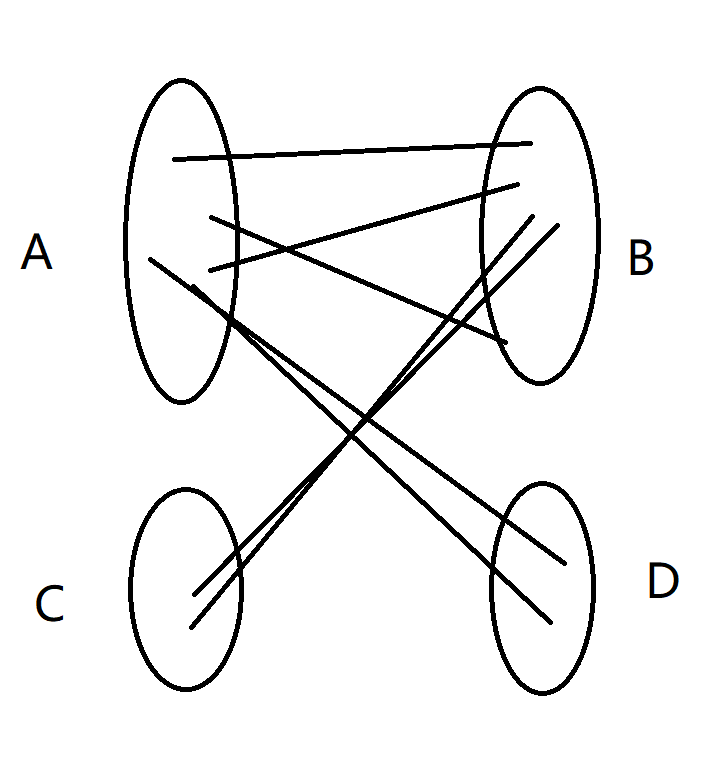
\includegraphics[width=0.8\textwidth]{p1.png}
 \end{center}
\paragraph{}Separating each side of the bipartite graph into two parts, part A and part B contain the points u with $\sum_{e \in E: u \in e} x_e =1$, part C and part D  contain the points u with $\sum_{e \in E: u \in e} x_e <1$. Apparently, if we want to maximize the cost, there will be no edge between part C and part D. Otherwise, the value of the edge can be larger and the new graph is still following the conditions.
 \begin{center}
  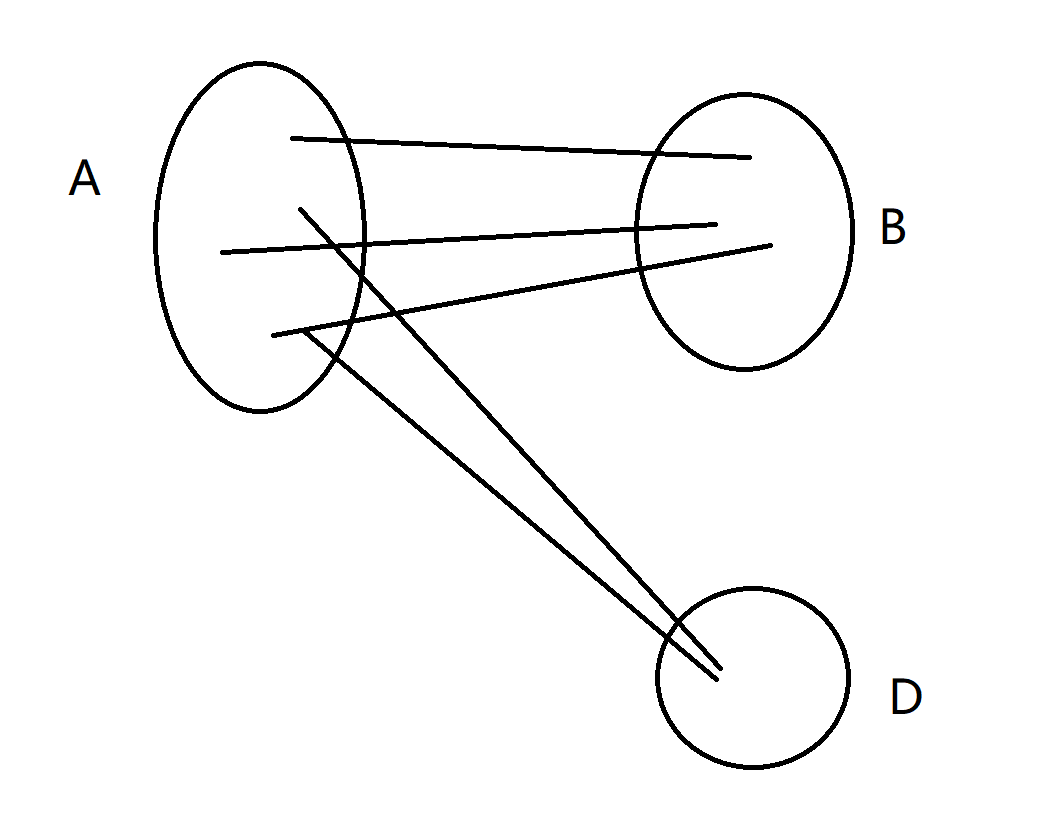
\includegraphics[width=0.8\textwidth]{p2.png}
 \end{center}
\paragraph{}Actually, part C or part D can be eliminated by finding some augmenting paths. Without the loss of generality, the graph would be like above.
\paragraph{}Finally, using the Hall's theorem, we know that $\nu(G) = |A|$. At the same time, $ \val(\textrm{MLP}(G)) = |A|$, too. So we've got $\nu(G) = \val(\textrm{MLP}(G))$
\begin{exercise}
  We know that $\nu(G) = \tau(G)$ for all bipartite graphs (K\H{o}nig's Theorem) and
  $\nu(G) \leq \tau(G)$ for all graphs (since every matched edge must be covered
  by a distinct vertex). Show that $\tau(G) \leq 2 \, \nu(G)$ for all graphs $G$.   
  
\paragraph{Solution.}

For a fixed max matching of $G$, it has $\nu(G)$ edges and $2\nu(G)$ vertices in it. Since the matching is the max matching of $G$, there won't be any edge between the vertices which are not in the matching, otherwise we could have a larger matching. 

So, edges outside the matching must have the form that it connects one vertex in the matching and one vertex outside the matching. As long as we choose every vertex in the matching, it must cover all the edges in $G$ which have the size $2\nu(G)$ and the max vertex cover must have a equal or smaller size.

Thus, we have $\tau(G) \leq 2 \, \nu(G)$ for all graphs $G$.

\end{exercise}

\begin{exercise}
   Show that $\tau(G) \leq 2\, \opt(\textrm{VCLP}(G))$ for all graphs $G$ (including non-bipartite graphs).
\end{exercise}
    We denote $\y$ be an optimal solution of this problem, and we find all the vertices which has a value larger than 1/2 in $V$, and we denote them as a set: $C:=\{v \in V | y_v \ge \frac{1}{2}\}$. For each edge $e = \{u, v\}$, because we should satisfy the constraint that $y_v + y_u \ge 1$, so there must be an endpoint of each edge in the set C. So C is a vertex cover, so $|C| \ge \tau (G)$.
    Then according to the definition of C, we have
    $$|c|=\sum_{v\in C}\mathbf{1} \le 2\sum_{v\in C}\mathbf{y_v} \le 2\sum_{v\in V}\mathbf{y_v} = 2val(\y) = 2 opt(VCLP(G))$$.
    Thus, $\tau(G) \le |C| \le 2 opt(VCLP(G))$
\begin{exercise}
\end{exercise}
\paragraph{Solution.}

1. $G = \{ [4], \{\{1,2\}, \{2,3\}, \{1,3\},\{1,4\}\}\}$.

2.$G = \{ [4], \{\{1,2\}, \{2,3\}, \{1,3\},\{1,4\}, \{2,4\}, \{3,4\}\}\}$

3. In VCLP and MLP, we have
\begin{align*}
    \sum_{u\in V} y_u
    &\geq \sum_{u\in V} y_u \sum_{u \in e, e \in E} x_e \\
    &= \sum_{e \in E, e = \{u, v\}} x_e (y_u + y_v) \\
    &\geq \sum_{e \in E} x_e
\end{align*}

Because $G$ is VCLP exact, we can let $y_u = 1$ for all $u \in Y$, and $y_u = 0$ for all $u \not\in Y$. 
But we have $ \sum_{u\in V} y_u = \sum_{e \in E} x_e$, so $y_u + y_v = 1$ or $x_e = 0$ satisfy. Hence $x_e = 0$
if $e \in Y$.

4. Let $H = (V, \{(u, v) : (u, v) \in E, u \in Y, v \in V / Y\})$, we can proof $H$ staisfy Hall condition. Because $G$ is VCLP exact, so we can let $y_u = 1$ for all $u \in Y$, and $y_u = 0$ for all $u \not\in Y$.
If any set $A \in Y$, .s.t 
$|\mathcal{N}(A)| < |A|$, then we can decrease the $y_u$ for $u \in A$ and increase $y_u \in \mathcal{N}(A)$ to get a smaller solution 
for VCLP, it leads a contradiction. So $H$ has a matching of size $|Y|$, $H$ is a subgraph of $G$. Than $|Y| = \nu(G) \leq \nu_f(G)=\tau_f(G)\leq\tau(G)=|Y|$, hence $G$ is 
MLP exact.
\end{document}